\iffalse
\documentclass[journal,12pt,onecolumn]{IEEEtran}
\usepackage{cite}
\usepackage{amsmath,amssymb,amsfonts,amsthm}
\usepackage{algorithmic}
\usepackage{graphicx}
\usepackage{textcomp}
\usepackage{xcolor}
\usepackage{txfonts}
\usepackage{listings}
\usepackage{enumitem}
\usepackage{mathtools}
\usepackage{gensymb}
\usepackage{comment}
\usepackage[breaklinks=true]{hyperref}
\usepackage{tkz-euclide} 
\usepackage{listings}
\def\inputGnumericTable{}                                 
\usepackage[latin1]{inputenc}                                
\usepackage{color}                                            
\usepackage{array}                                            
\usepackage{longtable}                                       
\usepackage{calc}                                             
\usepackage{multirow}                                         
\usepackage{hhline}                                           
\usepackage{ifthen}                                           
\usepackage{lscape}
\usepackage{caption}
\usepackage{subfigure}
\usepackage{gvv}
\usepackage{pgfplots}
\usepackage{circuitikz}
\usepackage{graphicx}

% Define \phase command
\newcommand{\phase}[1]{\text{arg}\left(#1\right)}

\newtheorem{theorem}{Theorem}[section]
\newtheorem{problem}{Problem}
\newtheorem{proposition}{Proposition}[section]
\newtheorem{lemma}{Lemma}[section]
\newtheorem{corollary}[theorem]{Corollary}
\newtheorem{example}{Example}[section]
\newtheorem{definition}[problem]{Definition}
\newcommand{\BEQA}{\begin{eqnarray}}
\newcommand{\EEQA}{\end{eqnarray}}
\newcommand{\system}[1]{\stackrel{#1}{\rightarrow}}
\newcommand{\define}{\stackrel{\triangle}{=}}
\theoremstyle{remark}
\newtheorem{rem}{Remark}

\begin{document}

\bibliographystyle{IEEEtran}
\vspace{3cm}

\title{Gate-2022-EE-58}
\author{EE22BTECH11008 - Annapureddy Siva Meenakshi$^{*}$}
\maketitle
\bigskip

\renewcommand{\thefigure}{\theenumi}
\renewcommand{\thetable}{\theenumi}
Q: Consider an ideal full-bridge single-phase DC-AC inverter with a DC bus voltage magnitude of $1000 V$. The inverter output voltage $v(t)$ shown below is obtained when diagonal switches of the inverter are switched with $50\%$ duty cycle. The inverter feeds a load with a sinusoidal current given by $i(t) = 10 \sin(\omega t - \frac{\pi}{3}) \, \mathrm{A}$, where $\omega=\frac{2\pi}{T}$. The active power, in watts, delivered to the load is \underline{\quad}.[Gate2022-EE-58]  \\     
\begin{figure}[htb]
  \centering
  \begin{tikzpicture}
  \begin{axis}[
    xlabel={$t$},
    ylabel={$v(t)$},
    axis lines=middle,
    ymin=-1.5, ymax=1.5,
    xtick={0,0.5,1.0,1.5},
    xticklabels={0, $0.5 T$, $1.0 T$, $1.5 T$},
    ytick={0},
    grid=none,
    enlargelimits=0.2,
    xticklabel style={xshift=-0.4cm},
    height=6cm,
    ]
    \addplot[const plot, thick, blue] coordinates {(0,1) (0.5,1) (0.5,-1) (1,-1) (1,1) (1.5,1)};
  \end{axis}
\end{tikzpicture}




  \label{fig:EE_58_f1}
\end{figure}
   

\solution
\fi
\begin{table}[!ht]
    \centering
        \begin{tabular}{|c|c|c|} 
    \hline
    \textbf{Variable} & \textbf{Description} & \textbf{Value} \\
    \hline
    $V_\text{s}$ & input DC voltage & $1000V$ \\
    \hline
    $i(t)$ & output current & $\sin(\omega t-\frac{\pi}{3})$ \\
    \hline
    $v(t)$ & Output voltage & given \\
    \hline 
    $\omega$& Frequency &  $\frac{2\pi}{T}$     \\
    \hline
       $v_{0}^{\text{rms}}$&  RMS output voltage at the fundamental frequency& none\\
    \hline
    $i_{\text{rms}}$&  RMS output current at the fundamental frequency& none\\
    \hline
     $v_{0}(t)$&  output voltage at the fundamental frequency& none\\
    \hline
    $\phi$ & phase difference between $v_{0}(t)$ and $i(t)$&none\\
    \hline
    $i_{0}$& amplitude of output current & $1$\\
    \hline
    $P$&        active power delivered&none\\
    \hline
\end{tabular}

    \caption{Input parameters}
    \label{tab:EE_58_t1}
\end{table}

\begin{figure}[htb]
  \centering
  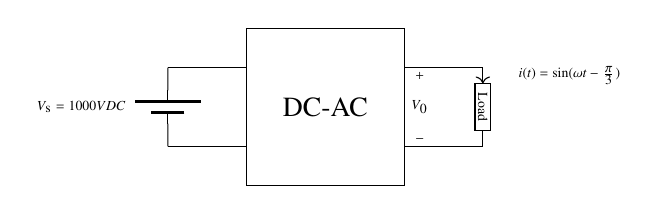
\begin{tikzpicture}

% Draw rectangle for inverter
\draw (0,0) rectangle (2,2);
\node at (1,1) {DC-AC};

% Draw input lines with battery
\draw (-1,1.5) -- (0,1.5) node[midway, left] {};
\draw (-1,0.5) -- (0,0.5) node[midway, left] {};

% Draw output lines
\draw (2,1.5) -- (3,1.5) node[right] {};
\draw (2,0.5) -- (3,0.5) node[right] {};

% Draw load resistor symbol with rotated text
\draw (2.9,0.7) rectangle (3.1,1.3) node[midway, rotate=90] {\rotatebox{-180}{\tiny Load}};

\draw (3,1.3) -- (3,1.5) node[right] {};
\draw (3,0.5) -- (3,0.7) node[right] {};

% Draw battery symbol without arrow and label
\draw (-1,1.5) to [battery1] (-1,0.5);
\node at (-2.1,1) {\tiny $V_\text{s}=1000V DC$};

% Draw current arrow
\draw[->] (3,1.5) -- (3,1.3) node[midway, above] {};

% Add labels for the current arrow
\node at (4.1,1.4) {\tiny $i(t)=\sin(\omega t-\frac{\pi}{3})$};
\node at (2.2,1.4) {\tiny $+$};
\node at (2.2,1) {\tiny $V_0$};
\node at (2.2,0.6) {\tiny $-$};
\end{tikzpicture}


   \captionsetup{justification=centering, singlelinecheck=off}
  \caption{circuit diagram of the system}
  \label{fig:EE_58_f2}
\end{figure}

The Fourier series expansion of the given voltage $v(t)$ is,
\begin{align}
  v(t) &= \sum_{n=1,3,5,\ldots}^{\infty} \frac{4V_{\text{dc}}}{n\pi} \sin(n\omega t)\\
    v_{0}(t)&=  \frac{4V_{\text{dc}}}{\pi} \sin(\omega t)\\
    \therefore \quad \phi &= \frac{\pi}{3}\\
    v_{0}^{\text{rms}}&=  \frac{4V_{\text{dc}}}{\pi \sqrt{2}}\\
    &=\frac{4000}{\pi \sqrt{2}}\\
    i_{\text{rms}}&=\frac{i_{0}}{\sqrt{2}}=\frac{1}{\sqrt{2}}
\end{align}
  Active power delivered to load in Watts is given by,
  \begin{align}
    P &= v_{0}^{\text{rms}} \times i_{\text{rms}} \times \cos{\phi}\\
    &= \frac{4000}{\pi \sqrt{2}} \times \frac{1}{\sqrt{2}} \times \cos{\frac{\pi}{3}}\\
    &\approx 3183 
\end{align}

\begin{figure}[htb]
  \centering
  \begin{tikzpicture}
    \begin{axis}[
      xlabel={$\omega t$},
      ylabel={$v_0(t)$},
      axis lines=middle,
      ymin=-1.5, ymax=1.5,
      xtick={0,0.5,1.0,1.5},
      xticklabels={0},
      ytick={0},
      grid=none,
      enlargelimits=0.2,
      xticklabel style={xshift=-0.4cm},
      width=8cm,
      height=6cm,
      ]
      \addplot[thick, black] coordinates {(0,1) (0.5,1) (0.5,-1) (1,-1)(1,0)};
      % Place Vs label at the right position
      \node at (axis cs:0.25,0.5) {$V_s$};
      \node at (axis cs:0.75,-0.5) {$-V_s$};
      
      % Vertical dotted line at x=0.5
      \draw[dotted] (axis cs:0.5, -1.5) -- (axis cs:0.5, 1.5);
      \draw[dotted] (axis cs:1, -1.5) -- (axis cs:1, 1.5);
    \end{axis}
  \end{tikzpicture}
  

   \captionsetup{justification=centering, singlelinecheck=off}
  \caption{output voltage and current of the system}
  \label{fig:EE_58_f3}
\end{figure}
\begin{figure}[htb]
  \centering
  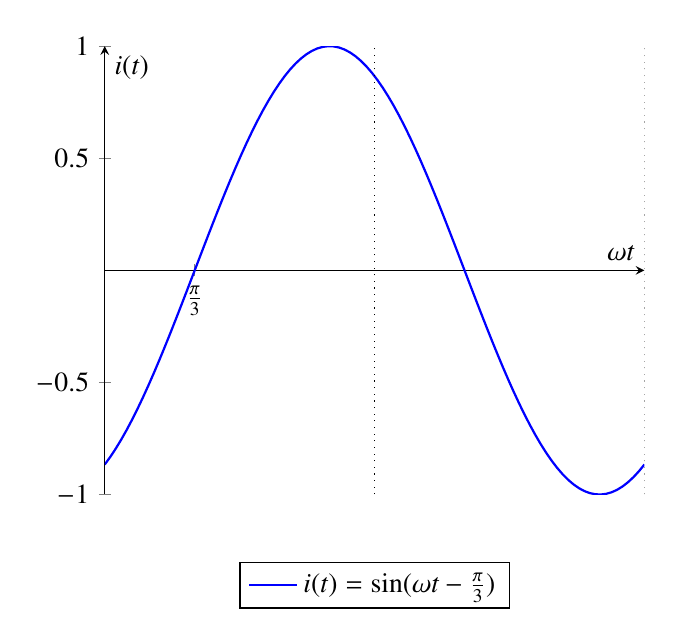
\begin{tikzpicture}

% Adjust the domain and samples according to your preference
\begin{axis}[
    xlabel={$\omega t$},
    ylabel={$i(t)$},
    domain=0:2*pi,
    samples=100,
    axis lines=middle,
    xtick={pi/3}, % Set x-axis tick at pi/3
    xticklabels={$\frac{\pi}{3}$}, % Label for the tick
    ytick={}, % Remove y-axis ticks
    legend style={at={(0.5,-0.15)},anchor=north},
]

% Plot the function
\addplot[blue,thick] {sin(deg(x - pi/3))};
\addlegendentry{$i(t) = \sin(\omega t - \frac{\pi}{3})$}

% Dotted vertical lines at x=pi and x=2pi
\draw[dotted] (axis cs:pi, \pgfkeysvalueof{/pgfplots/ymin}) -- (axis cs:pi, \pgfkeysvalueof{/pgfplots/ymax});
\draw[dotted] (axis cs:2*pi, \pgfkeysvalueof{/pgfplots/ymin}) -- (axis cs:2*pi, \pgfkeysvalueof{/pgfplots/ymax});

\end{axis}

\end{tikzpicture}

   \captionsetup{justification=centering, singlelinecheck=off}
  \caption{output voltage and current of the system}
  \label{fig:EE_58_f3}
\end{figure}
%\end{document}

